\documentclass{tufte-handout}

%\geometry{showframe}% for debugging purposes -- displays the margins

\usepackage{amsmath}

% Set up the images/graphics package
\usepackage{graphicx}
\setkeys{Gin}{width=\linewidth,totalheight=\textheight,keepaspectratio}
\graphicspath{{graphics/}}
\DeclareGraphicsExtensions{.pdf,.jpg,.png}

\title{The Uber Demand Prediction Challenge}
\author[Michael Sachs]{Michael Sachs}
\date{}  % if the \date{} command is left out, the current date will be used

% The following package makes prettier tables.  We're all about the bling!
\usepackage{booktabs}

% The units package provides nice, non-stacked fractions and better spacing
% for units.
\usepackage{units}

% The fancyvrb package lets us customize the formatting of verbatim
% environments.  We use a slightly smaller font.
\usepackage{fancyvrb}
\fvset{fontsize=\normalsize}

% Small sections of multiple columns
\usepackage{multicol}

% Provides paragraphs of dummy text
\usepackage{lipsum}

%\usepackage[tight,normalsize,sf,SF]{subfigure}

% These commands are used to pretty-print LaTeX commands
\newcommand{\doccmd}[1]{\texttt{\textbackslash#1}}% command name -- adds backslash automatically
\newcommand{\docopt}[1]{\ensuremath{\langle}\textrm{\textit{#1}}\ensuremath{\rangle}}% optional command argument
\newcommand{\docarg}[1]{\textrm{\textit{#1}}}% (required) command argument
\newenvironment{docspec}{\begin{quote}\noindent}{\end{quote}}% command specification environment
\newcommand{\docenv}[1]{\textsf{#1}}% environment name
\newcommand{\docpkg}[1]{\texttt{#1}}% package name
\newcommand{\doccls}[1]{\texttt{#1}}% document class name
\newcommand{\docclsopt}[1]{\texttt{#1}}% document class option name

\begin{document}
\maketitle

\newthought{The Uber} demand prediction challenge is the classic problem of predicting future events given some past data. Anyone who has tried to do this for say, the stock market, knows that getting meaningful results can be tricky. Not surprisingly success depends on the regularity of the past data. Below I describe a simple technique for making predictions of future demand on Uber's services given two months of past data. This technique is based mostly on patterns picked out from the data by eye. However, I also describe some more advanced pattern recognition techniques and how they can be applied to Uber data. 



\section{The Data}

%page images have a width of 6.3109in
\begin{figure*}[h]
    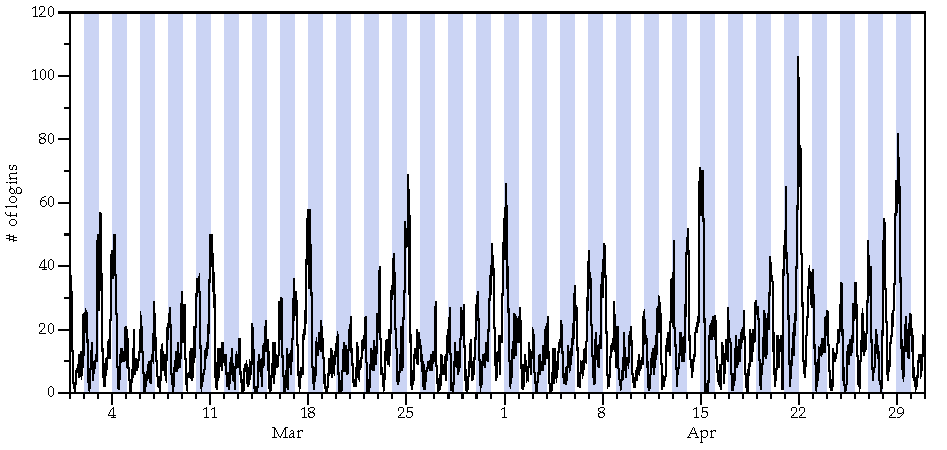
\includegraphics[width=\linewidth]{logins_per_hour.pdf}%
	\caption{The logins per hour for the two months of data provided.}%
	\label{fig:lph}%
\end{figure*}

The data provided for this challenge was a series of timestamps representing login times for Uber users. In order to make sense of this data, I parsed it into a time-series of logins per unit time. Several examples are shown in Figures \ref{fig:lph}, \ref{fig:lpd}, and \ref{fig:lpm}. Although each of these time-series have interesting features, the one that I used for the analysis that follows was the logins per hour (Figure \ref{fig:lph}). A detail of the logins per hour for the two week period ending on Sunday, April 22nd is shown in Figure \ref{fig:lph2week}. There are many interesting features in this time-series data. The first thing that stands out is that the data are periodic. There is a strong daily cycle with peaks around midnight and troughs around 8am. Clearly Uber is more popular with the bar crowd than with commuters. There is also a weekly cycle which peaks Saturday night. Again this is most likely a bar-crowd effect. 

There is another interesting feature that only shows up in Figure \ref{fig:lph}. It seems there are more logins (especially at peak times) closer to the end of each month. Why this happens is not entirely clear. The data do come from the Washington DC area, so perhaps it has something to do with the pay-day schedules of government employees. However, with only two months of data, it is hard to say whether this is part of an underlying process or just a random fluctuation.

%body images have a width of 3.987in
\begin{figure}[h]
	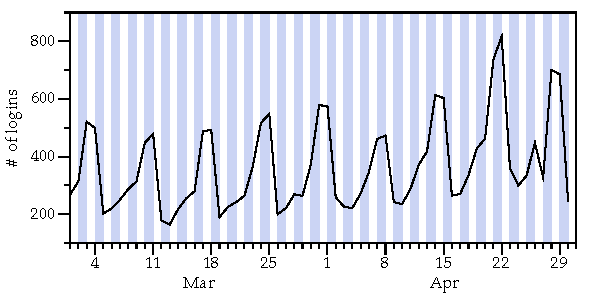
\includegraphics[width=\linewidth]{logins_per_day.pdf}%
	\caption{The logins per day for the two months of data provided.}%
	\label{fig:lpd}%
\end{figure}

%body images have a width of 3.987in
\begin{figure}[h]
	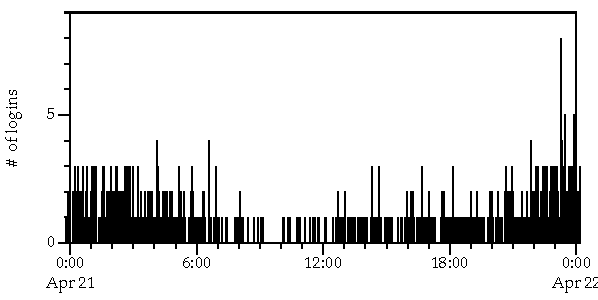
\includegraphics[width=\linewidth]{logins_per_minute.pdf}%
	\caption{The logins per minute for Saturday, April 21st 2012. This was the busiest day in the dataset.}%
	\label{fig:lpm}%
\end{figure}

%page images have a width of 6.3109in
\begin{figure*}[h]
    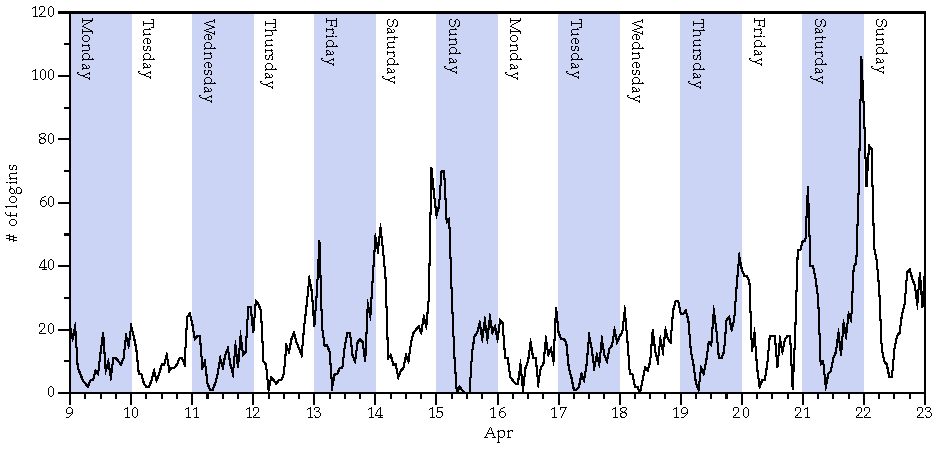
\includegraphics[width=\linewidth]{logins_per_hour_two_weeks.pdf}%
	\caption{The logins per hour for the two weeks ending on Sunday, April 22nd. The periodic structure is clear at this scale.}%
	\label{fig:lph2week}%
\end{figure*}

\section{The Forecasts}

The fact that the Uber login data has such a strong daily and weekly periodicity makes basic forecasting fairly simple. Because, for example, Monday, March 5 looks pretty much the same as Monday, April 2, it seems safe to assume that -- at least to first order -- this will hold for Monday, May 7. Building upon this similarity, my forecasting scheme simply averages each hour of each weekday over the number of instances of that weekday that appear in the data. So, taking Mondays as an example again, there are 9 Mondays in the data, therefore my forecast for Monday at 10am is the average of 9 values of Monday at 10am. This is expressed mathematically in Equation \ref{eq:forecast}:

\begin{equation}
        f_{hd} = \frac{\sum_d L_{hd}}{\sum_d}
        \label{eq:forecast},
\end{equation}

\noindent where $f$ if the forecast, $h$ and $d$ are the hour and day respectively, and $L$ is the login count. 

%page images have a width of 6.3109in
\begin{figure*}[h]
    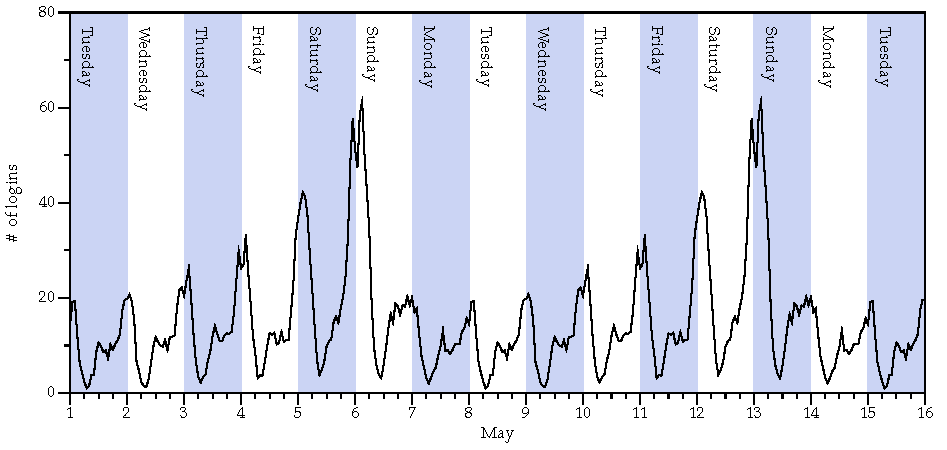
\includegraphics[width=\linewidth]{forecasts.pdf}%
	\caption{Forecast logins per hour for the time period May 1 2012 - May 15 2012. The daily and weekly periodic structure from Figure \ref{fig:lph2week} is captured in this forecast.}%
	\label{fig:forecasts}%
\end{figure*}

The results of applying this forecasting scheme are shown in Figure \ref{fig:forecasts}. The daily and weekly periodicity is clearly captured. The forecast shows high ``bar-time'' demand, especially on weekends, and low morning commute demand, exactly like the data. However, because the monthly effect that I described above is subtle -- and because there are only two months of data -- the forecast in Equation \ref{fig:forecasts} and Figure \ref{eq:forecast} does not include any monthly variations. This effect could be added by superimposing the monthly variations $M(t)$ in Equation \ref{eq:forecast}:

\begin{equation}
        f_{hd}(t) = \frac{\sum_d L_{hd}}{\sum_d} + M(t)
        \label{eq:forecast2}.
\end{equation}

\noindent The form of $M(t)$ could be inferred from the data or based on a model that captures the monthly dynamics.

\section{Further Explorations}

The forecast described above is effective but fairly basic. I was excited by the data, and wanted to explore some additional techniques that could be used to improve forecasting, but are also just interesting ways to look at time-series data. In what follows I am not drawing any conclusions or suggesting applications. I am merely poking around to see if I can find anything interesting.

\subsection{Fourier Transforms}

The first tool that is used in the analysis of any stationary time series is usually the Fourier transform. This technique is based on the fact that any discrete time series $X$ can be rewritten as a sum of sines and cosines (Equation \ref{eq:fourier_trans}).

\begin{equation}
        X_n = \sum_{n=0}^{N-1} x_n \exp^{-i2\pi k \frac{n}{N}}
        \label{eq:fourier_trans}.
\end{equation}

\noindent The $x_n$ are a measure of the amount, or power, of each frequency present in the signal. Equation \ref{eq:fourier_trans} can be inverted to extract the $x_n$ in terms of the $X_n$; this is a Fourier transform. The particular algorithm I used is the fast Fourier transform that is implemented as part of the python Numpy package, details can be found at \url{http://docs.scipy.org/doc/numpy/reference/routines.fft.html} and \citet{cooleyT65, pressTVF07}.

The results of the fast Fourier transform applied to the Uber logins per hour data (Figure \ref{fig:lph}) are shown in Figure \ref{fig:fft}. The top of Figure \ref{fig:fft} shows the normalized power over all periods in the data while the bottom focusses in on the region marked in blue. The first thing that pops out in Figure \ref{fig:fft} is the periodicity mentioned above. The strongest cycle is, as guessed, at the one day mark with the next strongest cycle at the 7 day mark. It is also interesting to note that my observation of a monthly cycle seems to also be correct with some power in the $\sim$30 and $\sim$60 day modes. Concentrating on the bottom plot of Figure \ref{fig:fft}, there are some other active modes that were not immediately apparent, particularly the power in the 0.5 day mode and the 3.5 day mode.

%body images have a width of 3.987in
\begin{figure}[h]
	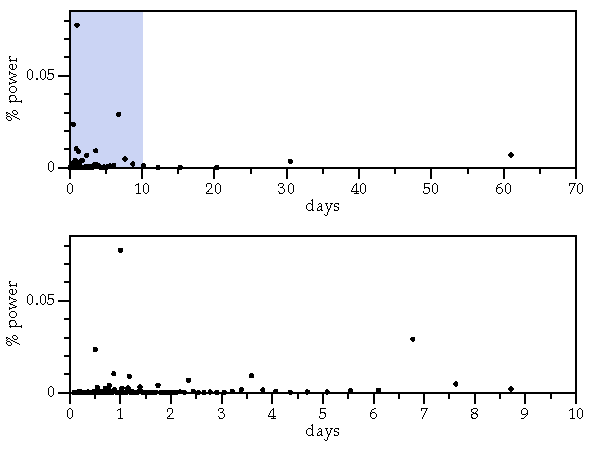
\includegraphics[width=\linewidth]{fft.pdf}%
	\caption{The normalized power spectrum of the Uber logins per hour time-series data. {\bf Top} The power spectrum for all periods in the data. {\bf Bottom} The power spectrum for the region marked in blue.}%
	\label{fig:fft}%
\end{figure}

\subsection{Frequency-Magnitude}

My dissertation work involved (among other things) looking at scaling relations in complex systems \citep{SachsYTRM12}. One particularly important scaling relation is the Gutenberg-Richter frequency-magnitude relation in seismology \citep{GutenbergR54}. This relation compares the cumulative number of earthquakes $N$ to their magnitudes $m$:

\begin{equation}
        \log N = a - b m
        \label{eq:gr},
\end{equation}

\noindent where $a$ and $b$ are constants. The basic idea is that for a certain number of small earthquakes (the exact number depending on the value of $b$), one can expect a large earthquake.

%body images have a width of 3.987in
\begin{figure}[h]
	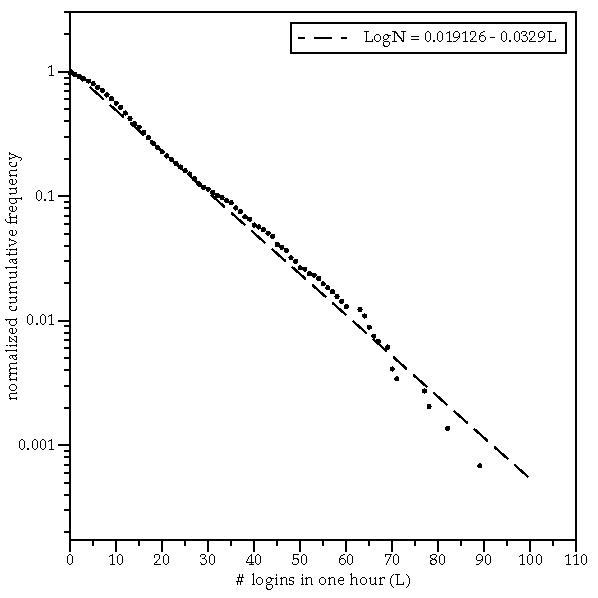
\includegraphics[width=\linewidth]{flc.pdf}%
	\caption{The cumulative frequency-login count for the Uber logins per hour data.}%
	\label{fig:flc}%
\end{figure}

The Uber login data inspired me to see what a ``frequency-login count'' relation looks like. The results are shown in Figure \ref{fig:flc}. The basic idea in this figure is that we are counting the number of hours that have login counts greater than or equal to the numbers listed on the x-axis. So, for example, around 40\% of the hours in the Uber data have 10 or more logins in them while only about 1\% have 50 or more. There is a nice linear relationship that is expressed in Figure \ref{fig:flc}:

\begin{equation}
        \log N = 0.019126 -0.0329 L
        \label{eq:gr}.
\end{equation}


Above about $L = 70$ there is a deviation from the linear relationship. This usually indicates some kind of change in the process that generates the data, although here it my just be due to the small sample size.

\subsection{Shannon Entropy}

The idea of entropy in information was first introduced by \citet{Shannon48} as a measure of the amount of information in a signal. It is usually defined as:

\begin{equation}
        H(X) = - \sum_i P(X_i) \log P(X_i)
        \label{eq:shannon_entropy}.
\end{equation}

\noindent In Equation \ref{eq:shannon_entropy}, $X$ is a discrete random variable, and $P(X_i)$ is the probability of the variable being $X_i$. The logarithm is usually taken as base two, which results in $H$ being in bits. Highly random signals will have a high entropy, while signals that are predictable will have a low entropy. The definition of entropy in Equation \ref{eq:shannon_entropy} can be difficult to apply to signals that are not binary. In order to avoid this difficulty a new definition called permutation entropy \citep{BrandtP02} can be employed. The permutation entropy is defined as:

\begin{equation}
        H(n) = - \sum_i p(\pi) \log p(\pi)
        \label{eq:permutation_entropy}.
\end{equation}

\noindent $p(\pi)$ is the probability of finding permutations $\pi$ of order $n$ in the signal. The logarithm is base two. For example: assume that our signal is $x = (4,7,9,10,6,11,3)$. Looking at each pair of numbers -- this is order $n = 2$ -- there are four pairs where the first number is smaller than the second. There are two pairs where the first number is bigger than the second. These are the only possibilities at $n = 2$. There are six total pairs. The permutation entropy is:

\begin{equation}
        H(2) = - \frac{4}{6} \log \frac{4}{6} - \frac{2}{6} \log \frac{2}{6} \simeq 0.918
        \label{eq:permutation_entropy_eg}.
\end{equation}

\noindent The permutation entropy in Equation \ref{eq:permutation_entropy} is bounded: $0 \leq H(n) \leq \log n!$. It is convenient to define a new value $h_n = H(n)/\log n! $ which is zero for a completely predictable signal and one for a completely random signal.

The results of applying this to the Uber logins per hour data are shown in Figure \ref{fig:pe}. Here $h_n$ was calculated for several values of $n$ on a moving window of $T_{win} = 336$ hours (two weeks). It can be tricky choosing the correct value of $n$ to use, if $n$ is too small the signal can look more random than it actually is, if $n$ is too high the signal may not have a representative number of permutations to sample. I have chosen $n = 6$ here (the bold line in Figure \ref{fig:pe}) because it retains some of the structure of the lower $n$ values but is still small enough to be reasonably well represented in the 336 hour sample. The first two weeks have $h_n = 0$ because of the value of $T_{win}$.


%body images have a width of 3.987in
\begin{figure}[h]
	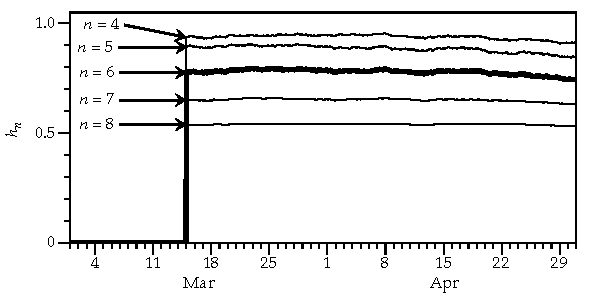
\includegraphics[width=\linewidth]{pe.pdf}%
	\caption{The permutation entropy $h_n$ calculated for various values of $n$ and a moving two week window ($T_{win} = 336$ hours). }%
	\label{fig:pe}%
\end{figure}

The first interesting feature in Figure \ref{fig:pe} is the fact that $h_n$ changes very little throughout the two month period. This again confirms that the dominant features of the original data are the daily and weekly cycles. Next, there does seem to be a dip towards the end of April. It is not clear if this is reflecting a longer term dynamic or if it is just noise.

\section{Epilogue}

Data from Uber's services are extremely interesting. I feel like I have only been able to scratch the surface of what is possible. I would love to explore how more than two months of data would change my results. Also, how would data from different cities compare? There is a trove of information here for cultural anthropologists. It would also be interesting to develop a more comprehensive model of transportation demand based on this data. Lastly, it would be fascinating to include geo-spatial data in these results.


\bibliography{/Users/sachs/Documents/BibTex/references.bib}
%\nobibliography{LaTeX_template}
\bibliographystyle{plainnat}

\end{document}